\documentclass{beamer}
\usetheme{Madrid}

\title{Tackling the curse of dimensionality}
\subtitle{one dimension at a time}
\author{Yon Ploj}
\institute{Univerza v Ljubljani, fakulteta za računalništvo in informatiko}
\date{May 2025}

\begin{document}

\frame{\titlepage}

\begin{frame}{Quick Recap}
\begin{itemize}
    \item Multi-asset Black-Scholes PDE for option pricing
    \item Curse of dimensionality: computational cost grows exponentially
    \item Physics-Informed Neural Networks (PINNs) as a solution
    \item Stochastic Dimension Gradient Descent (SDGD) to accelerate training
\end{itemize}
\end{frame}

\begin{frame}{Implementation}
\begin{itemize}
    \item Neural network architecture:
    \begin{itemize}
        \item Input: $n_{assets} + 1$ dimensions (prices + time)
        \item Two hidden layers with 16 neurons each
        \item Output: option price
    \end{itemize}
    \item Training process:
    \begin{itemize}
        \item Randomly sample subset of dimensions each epoch
        \item Calculate gradients only for selected dimensions
        \item Full loss calculation every 10 seconds
    \end{itemize}
\end{itemize}
\end{frame}

\begin{frame}{Synthetic Data Generation}
\begin{itemize}
    \item Two-step process:
    \begin{itemize}
        \item Generate model parameters (volatilities, correlations, etc.)
        \item Simulate price paths using geometric Brownian motion
    \end{itemize}
    \item Realistic parameters:
    \begin{itemize}
        \item Volatilities: 15\% to 35\%
        \item Correlations: -0.3 to 0.7
        \item Initial prices: 15.0 to 35.0
    \end{itemize}
    \item Added noise to simulate real-world imperfections
\end{itemize}
\end{frame}

\begin{frame}{Experimental Setup}
\begin{itemize}
    \item Tested various configurations:
    \begin{itemize}
        \item 3 assets: 1 and 3 dimensions per batch
        \item 30 assets: 1, 10, and 30 dimensions per batch
        \item 100 assets: 1, 5, and 100 dimensions per batch
    \end{itemize}
    \item Each experiment run for up to 1 hour
    \item Early stopping based on full-dimension loss
    \item Hardware: NVIDIA H100 GPU
\end{itemize}
\end{frame}

\begin{frame}{Results: Training Speed}
\begin{itemize}
    \item Smaller dimension batch sizes = faster learning
    \item Speedup increases with problem dimensionality
    \item More epochs needed, but less wall-clock time
\end{itemize}
\end{frame}

\begin{frame}{Results: Plots 1}
\begin{figure}
    \centering
    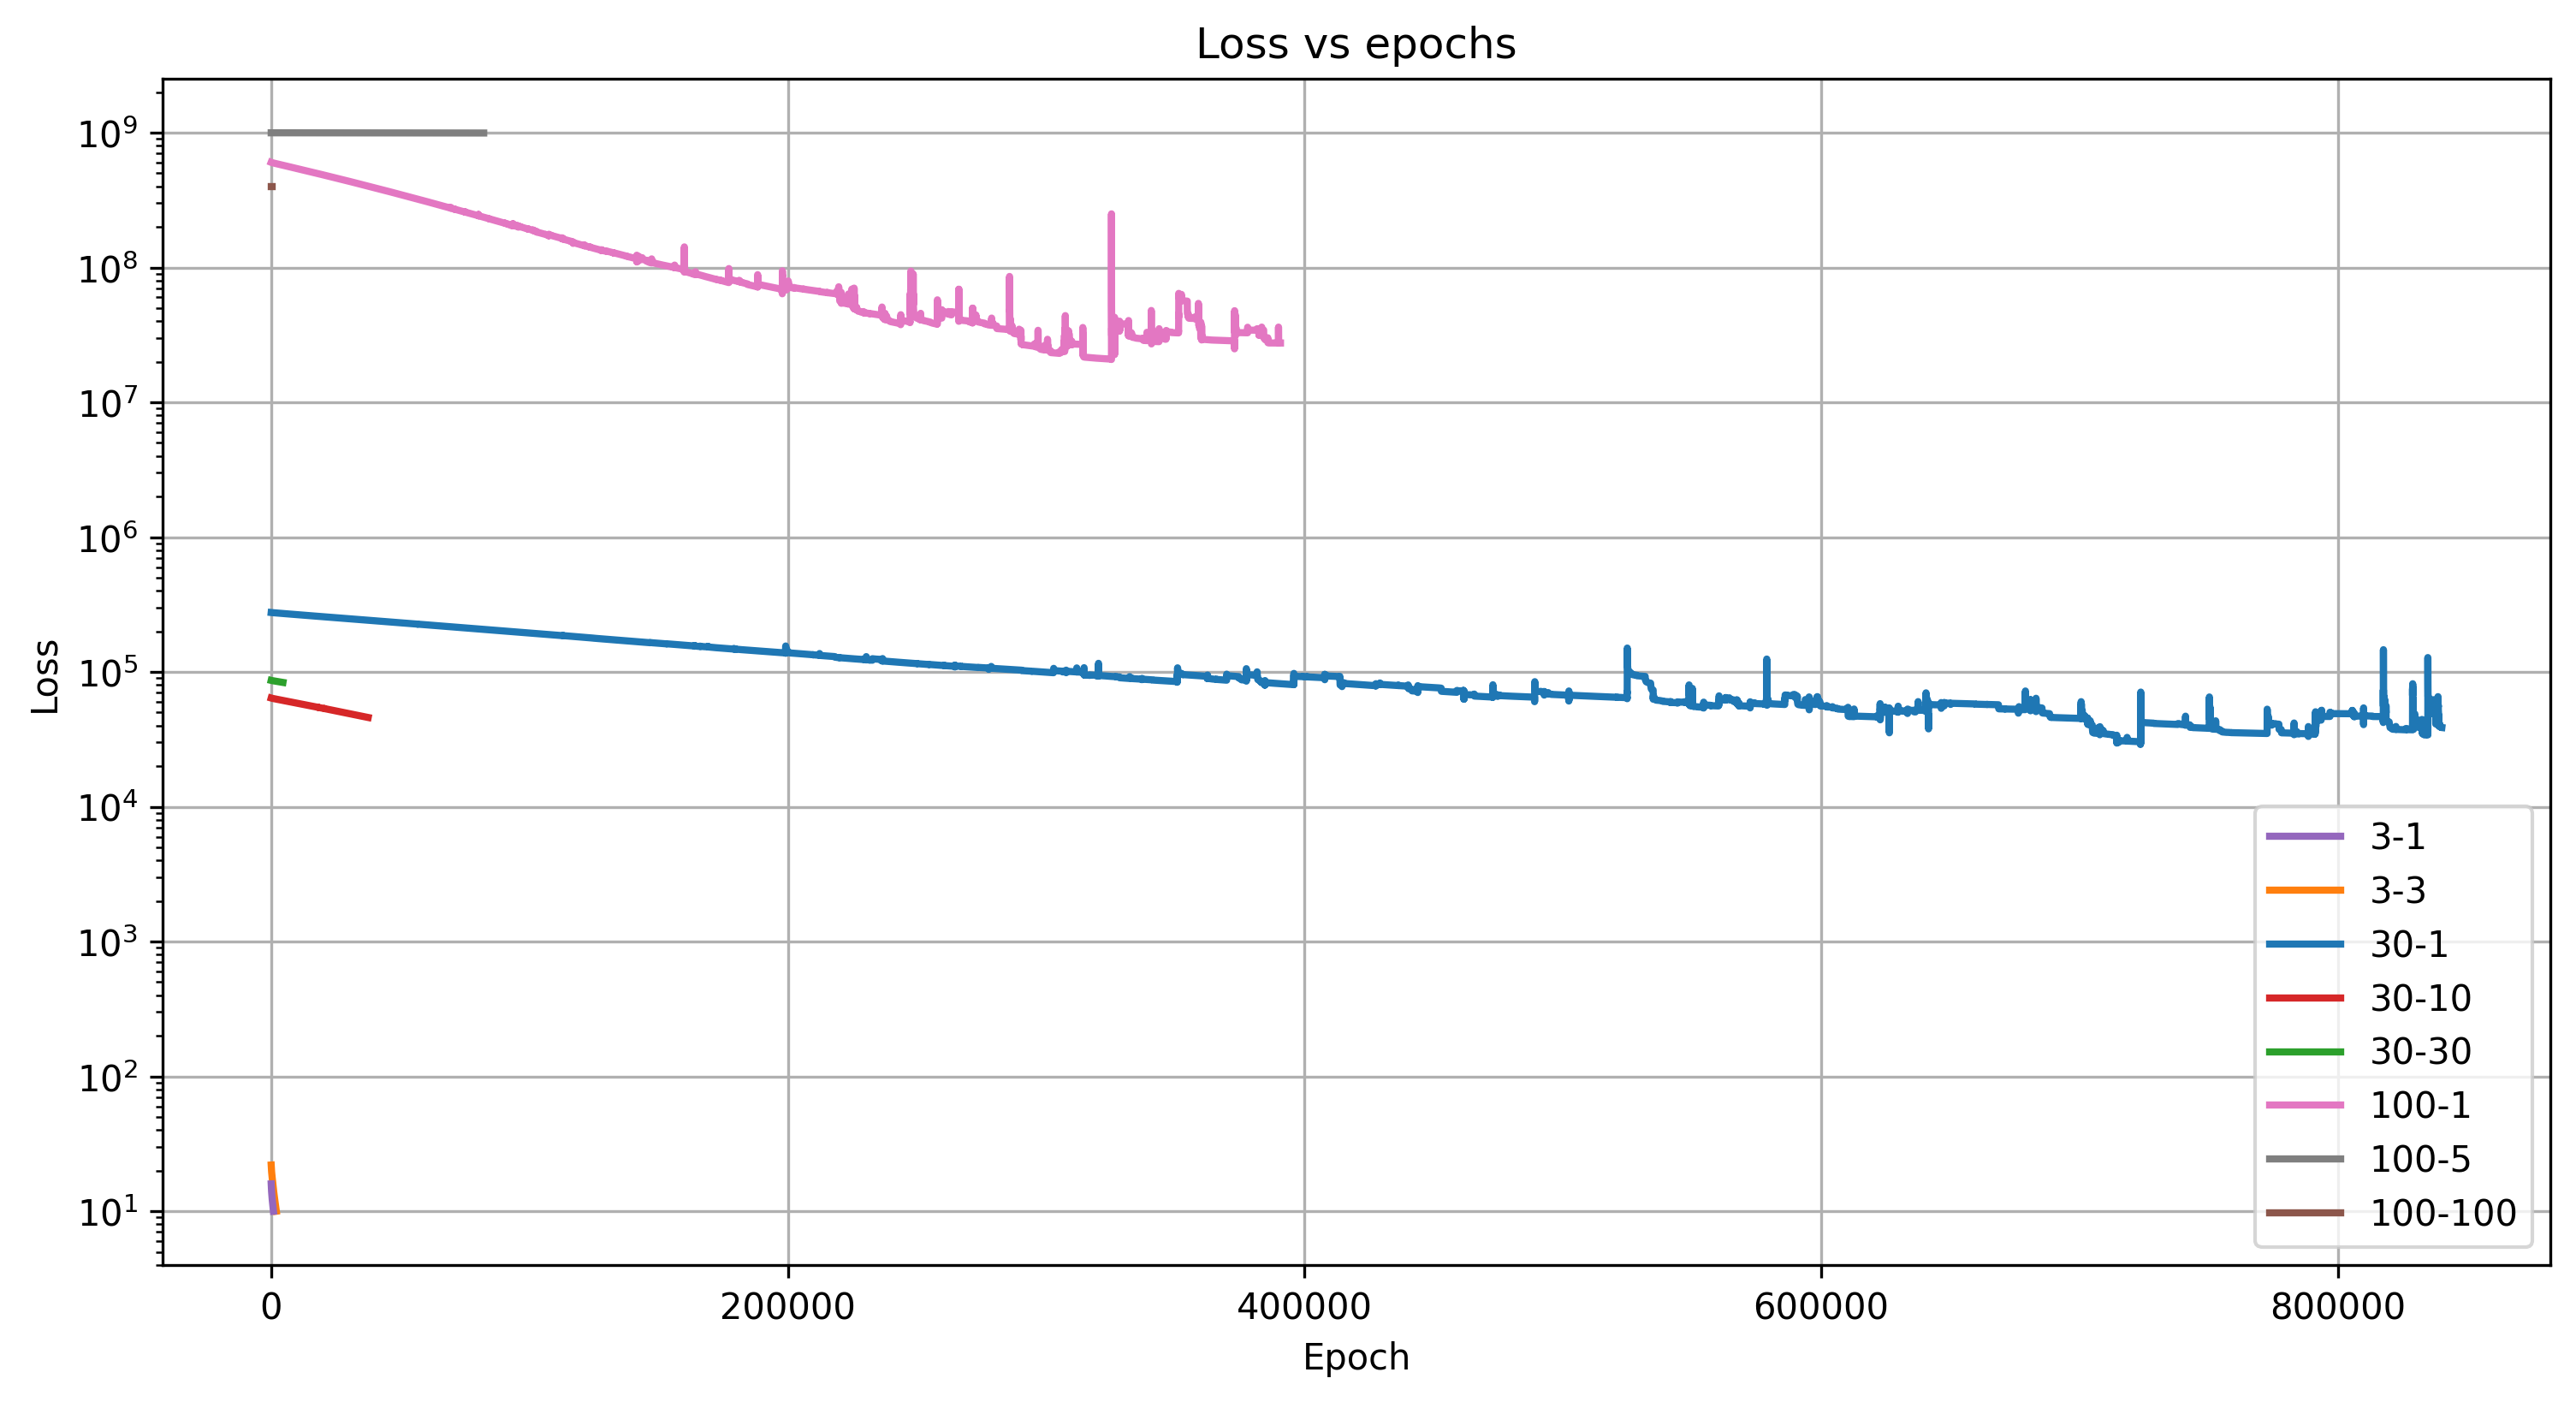
\includegraphics[width=1\linewidth]{loss_vs_epochs.png}
    \label{fig:enter-label}
\end{figure}
\end{frame}

\begin{frame}{Results: Plots 2}
\begin{figure}
    \centering
    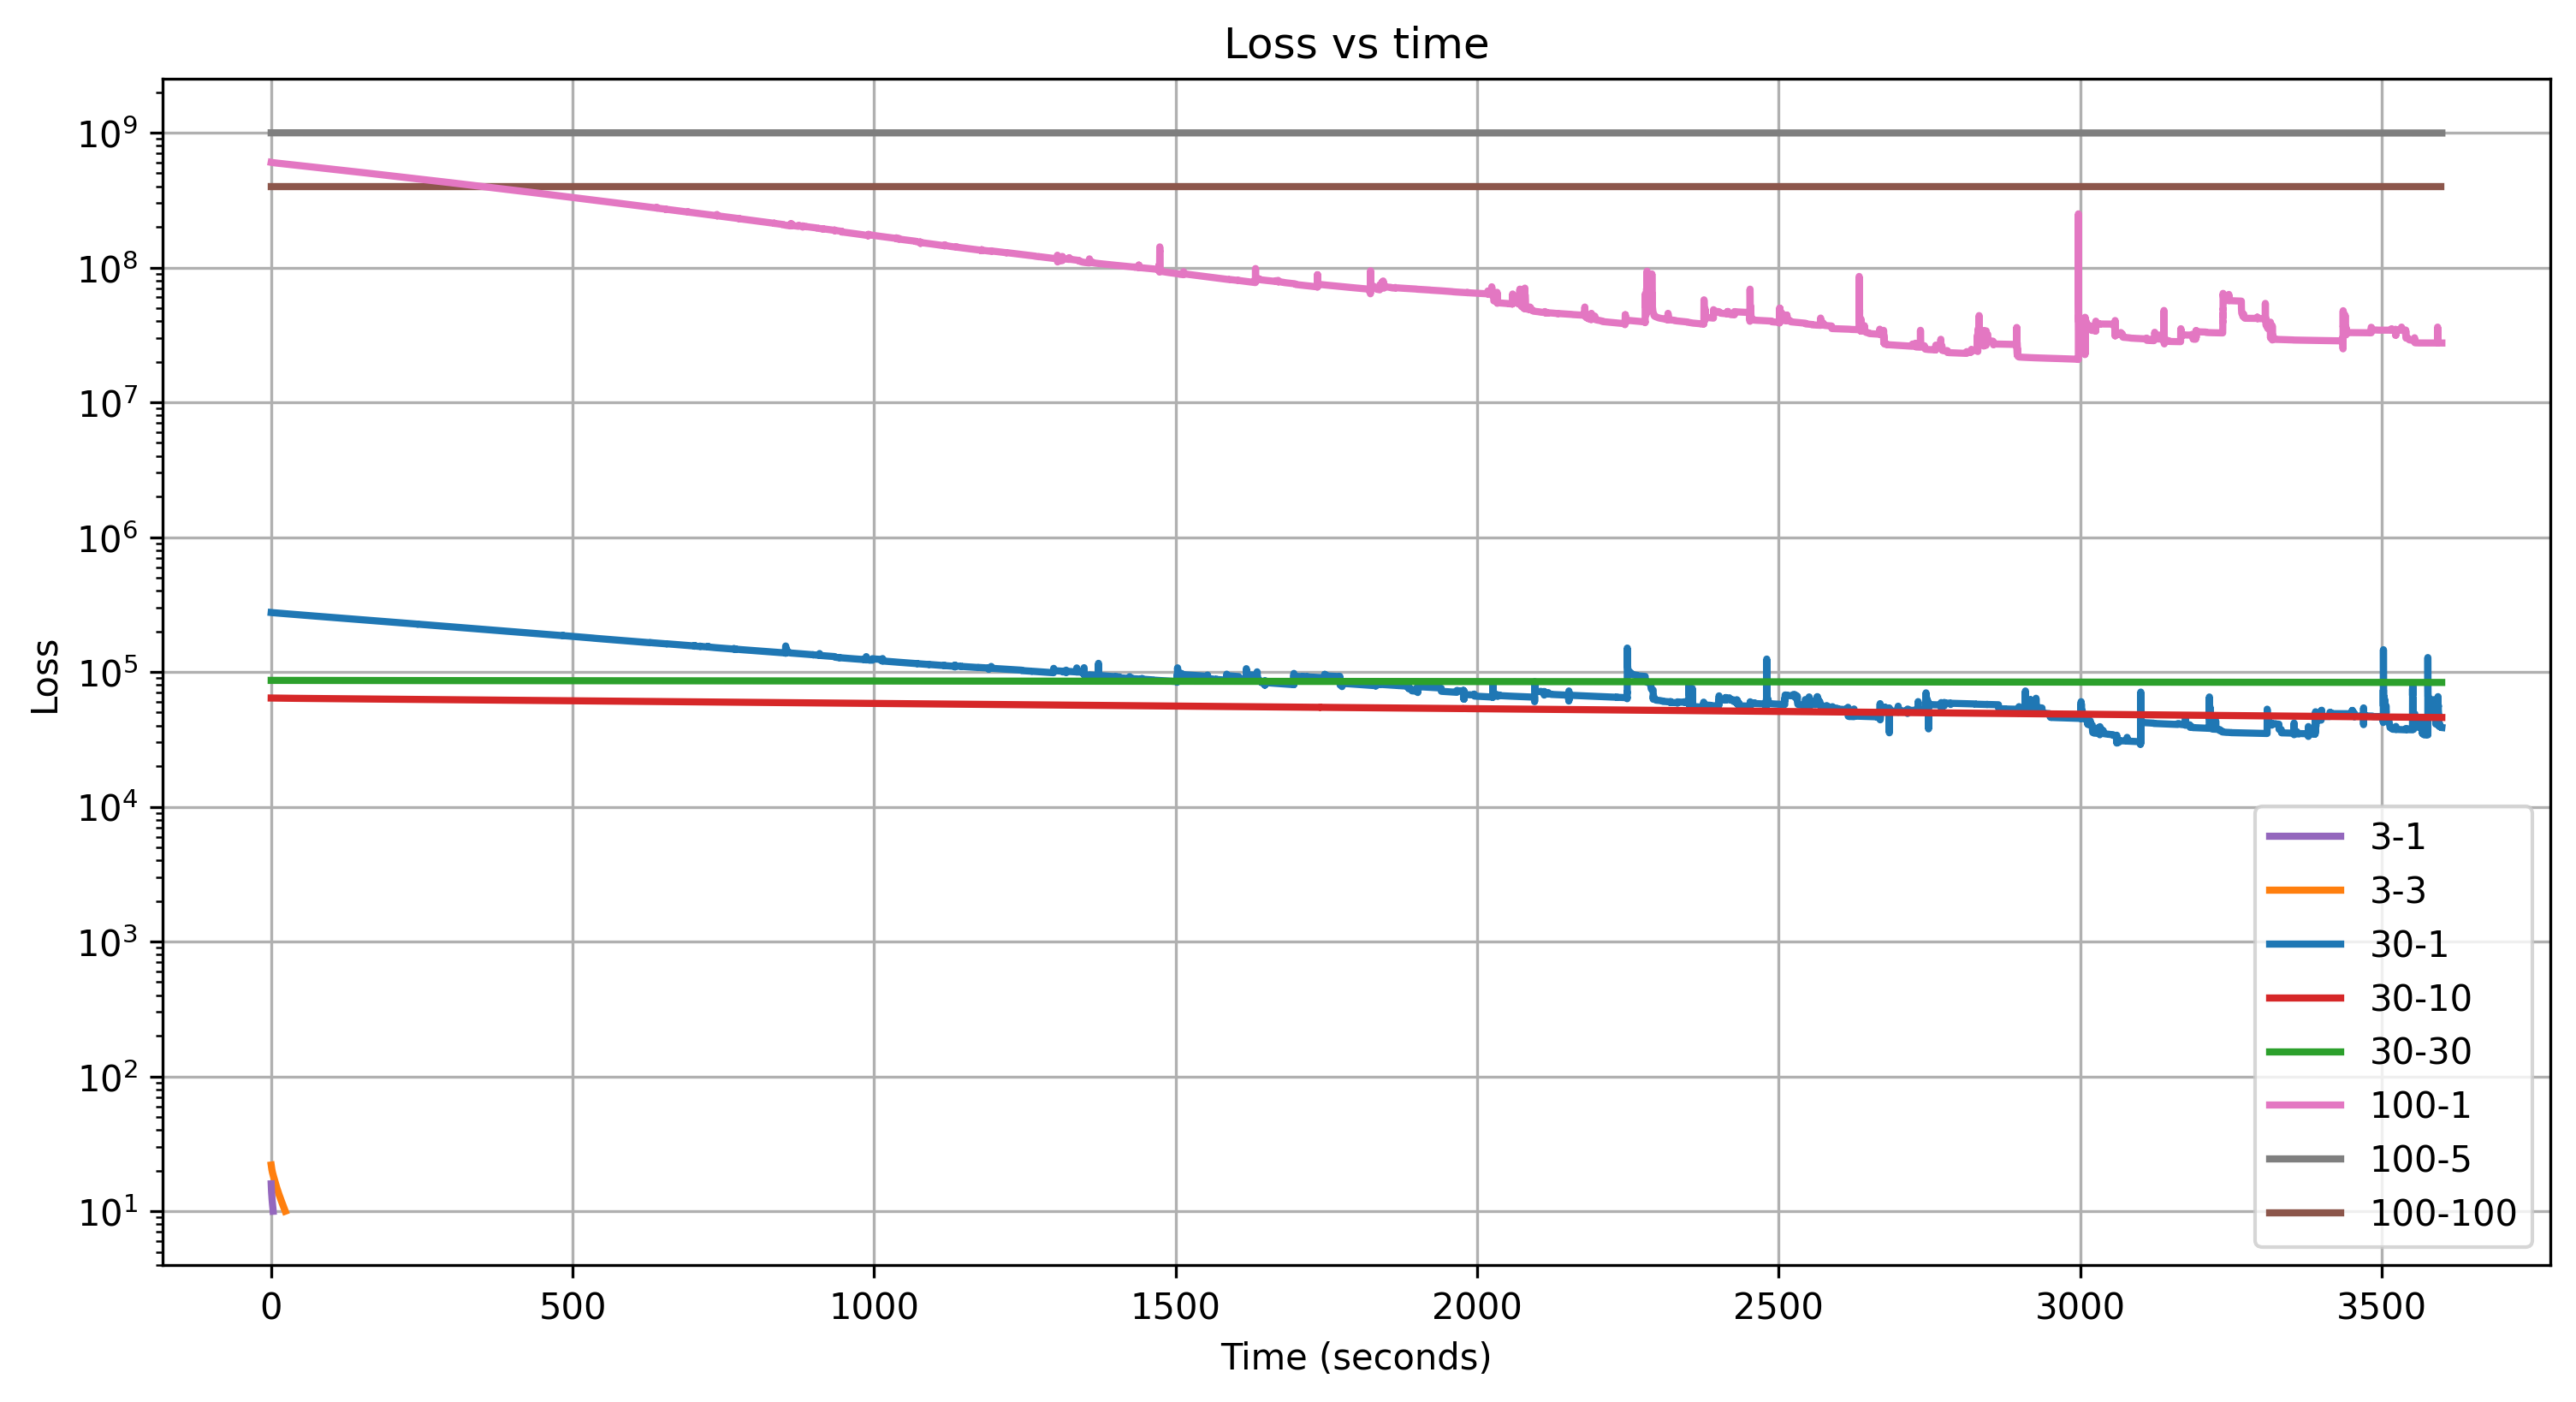
\includegraphics[width=1\linewidth]{loss_vs_time.png}
    \label{fig:enter-label}
\end{figure}
\end{frame}

\begin{frame}{Challenges and Limitations}
\begin{itemize}
    \item Gradient instability with smaller batch sizes
\end{itemize}
\end{frame}

\begin{frame}{Blank slide}
Thank you

\end{frame}

\end{document}
